
\section{Kernel Methods}
Motivation: solve issue of feature explosion (extreme dimensionality of data): \#training data= n + m-th degree polynomial features + $ \phi(x) \in R^d$  + $ x \in R^p$

\textbf{Dim of feature map $\phi(x)$:} $p = (d+m, m) = \frac{(d+m)!}{m!d!}$ $O(d^m) = f(d)$ and $O(m^d) = f(m)$, size of total training data = np

\textbf{Kernel trick}
Step I: global minimizer $\hat{w} = \arg \min_{w \in R^p} \frac{1}{n} \sum^{n}_{i=1}l(y_i, f_w(x_i))$ has the form $\hat{w} = {\phi}^T\hat{\alpha}$ with $\hat{\alpha} \in R^n$ so that $\hat{f}(x) = \sum^{n}_{i=1}\hat{\alpha}_i \langle  \phi(x_i), \phi(x) \rangle$ and where $\hat{\alpha}$ only depends on $x_i$ via inner products $\langle  \phi(x_i) , \phi(x_j) \rangle$ for $i, j = 1, ..., n$ (save memory $O(n{d^m}) \rightarrow O(n^2)$ - kernel matrix)\\
Step II: $\langle \phi(x), \phi(z) \rangle = (1 + \langle x,z \rangle)^m$ Efficient computation for the inner product of kernel function (from $O(p)\sim O(d^m)$ to $O(d+m)$) (kern.matr. $K$ has $n^2$ kernels comput. complex. $O((d+m)n^2)$)\\

\textbf{Kernelized regression}:
%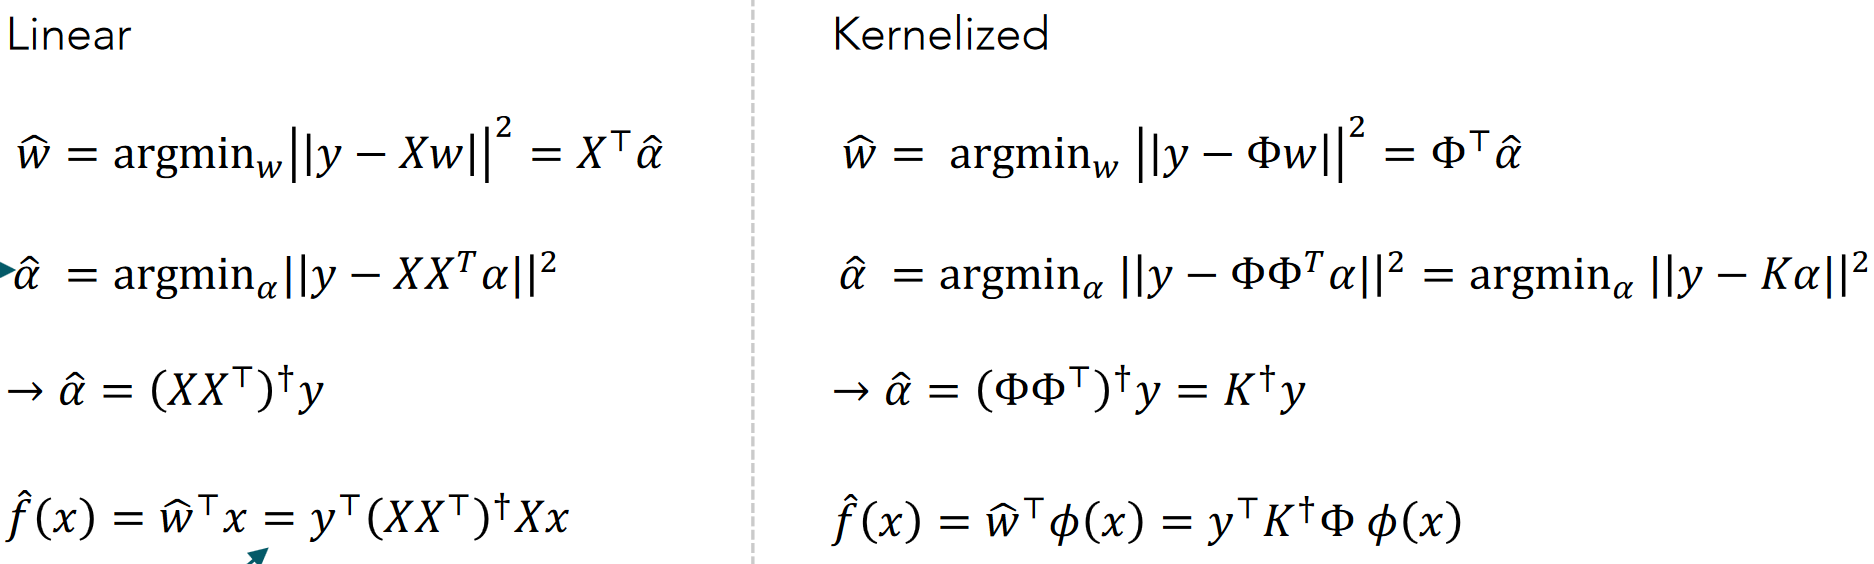
\includegraphics[width=\linewidth]{pics/figure7.PNG} \\
$\hat{w} = \arg \min_w ||y-\phi w||^2 = \phi^T \hat{\alpha}$ where $\hat{\alpha} = \arg \min_{\alpha}||y-\phi\phi^T\alpha||^2 = \arg \min_{\alpha} ||y-K\alpha||^2$\\
\textbf{Kernelized loss with ridge regularization}:
$\arg \min_{\alpha \in \mathbb{R}^n} ||y - K\alpha||^2 + \lambda {\alpha^T}K\alpha$\\
\textbf{Proof of kernel trick}:\\
Kernel trick can limit search from $R^d$ to $S$ ($S = span \{\phi(x_1), ..., \phi(x_n)\}$) \\
\textbf{Marcel's Theorem}: For kernels $k:X \times X \rightarrow R$ on a compact domain $X \in R^d$, $\exists$ sequence $\{\mu_j\}^{\infty}_{j=1}$ and basis $\{\phi_j\}^{\infty}_{j=1}$ of $L_2(X)$ (a sequence of functions) such that $k(x, y) = \sum^{\infty}_{j=1}\mu_j \phi_j(x)\phi_j(y) = \langle  \tilde{\phi}(x_j) , \tilde{\phi}(y_j) \rangle$ 

\textbf{Valid kernels} symmetric + psd: 
$min\{x, z\}$, 
const. $> 0$,  
$x^Tx'$, 
$|A \cap B|$, 
RBF kernels: $k(x, z) = e^{-\frac{||x-z||^{\alpha}}{\tau}}$, $\tau \downarrow$ overfit
(Gaussian: $\alpha = 2$\quad Laplacian: $\alpha = 1$)\\
\textbf{k-Nearest Neighbor}: can be kernelized\\
1. Sensitive to initialization (using cross-validation for choosing k);\quad
2. becomes erratic in high dimensions (all points become far);\quad 
3. needs large n to perform well but computation $O(nd)$, can reduce to $O(n^{\rho}), \rho < 1$ if allowing some error probability\\
\textbf{Decision trees}:
Leaf nodes of a binary tree. \textbf{But}
- can easily overfit to noise; - inaccurate as the greedy method








